% Author: Alfredo Sánchez Alberca (asalber@ceu.es)
\begin{tikzpicture}
\draw [vector] (0,0) node[anchor=south east]  {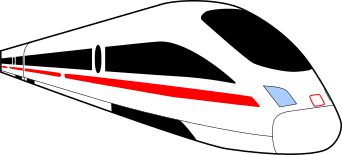
\includegraphics[scale=0.4]{img/analytic_geometry/train}} -- (2,-0.5) node[black, above, midway] {$\vec{v}$} node[sloped, pos=1, anchor=west] {direction};
\draw [decorate, decoration={brace, amplitude=5pt, mirror}, xshift=-2pt, yshift=-2pt] (0,0) -- (2,-0.5) node [midway, below, sloped, xshift=-2pt, yshift=-2pt] {magnitude};
\end{tikzpicture}
